\documentclass[a4paper,12pt]{article}

\usepackage[utf8x]{inputenc}
\usepackage[T2A]{fontenc}
\usepackage[english, russian]{babel}

% Опционно, требует  apt-get install scalable-cyrfonts.*
% и удаления одной строчки в cyrtimes.sty
% Сточку не удалять!
% \usepackage{cyrtimes}

% Картнки и tikz
\usepackage{graphicx}
\usepackage{tikz}
\usetikzlibrary{snakes,arrows,shapes}


% Некоторая русификация.
\usepackage{misccorr}
\usepackage{indentfirst}
\renewcommand{\labelitemi}{\normalfont\bfseries{--}}

% Увы, поля придётся уменьшить из-за листингов.
\topmargin -1cm
\oddsidemargin -0.5cm
\evensidemargin -0.5cm
\textwidth 17cm
\textheight 24cm

\sloppy

% Оглавление в PDF
\usepackage[
bookmarks=true,
colorlinks=true, linkcolor=black, anchorcolor=black, citecolor=black, menucolor=black,filecolor=black, urlcolor=black,
unicode=true
]{hyperref}

% Для исходного кода в тексте
\newcommand{\Code}[1]{\texttt{#1}}

\usepackage{verbatim}
\usepackage{fancyvrb}
\fvset{frame=leftline, fontsize=\small, framerule=0.4mm, rulecolor=\color{darkgray}, commandchars=\\\{\}}
\renewcommand{\theFancyVerbLine}{\small\arabic{FancyVerbLine}}


\title{Отчёт по лабораторной работе \\ <<IP-маршрутизация>>}
\author{Здесь Ф.~И.~О}

\begin{document}

\maketitle

\tableofcontents

% Текст отчёта должен быть читаемым!!! Написанное здесь является рыбой.

\section{Топология сети}

Топология сети и использыемые IP-адреса показаны на рис.~\ref{fig:network}.

\begin{figure}
\centering
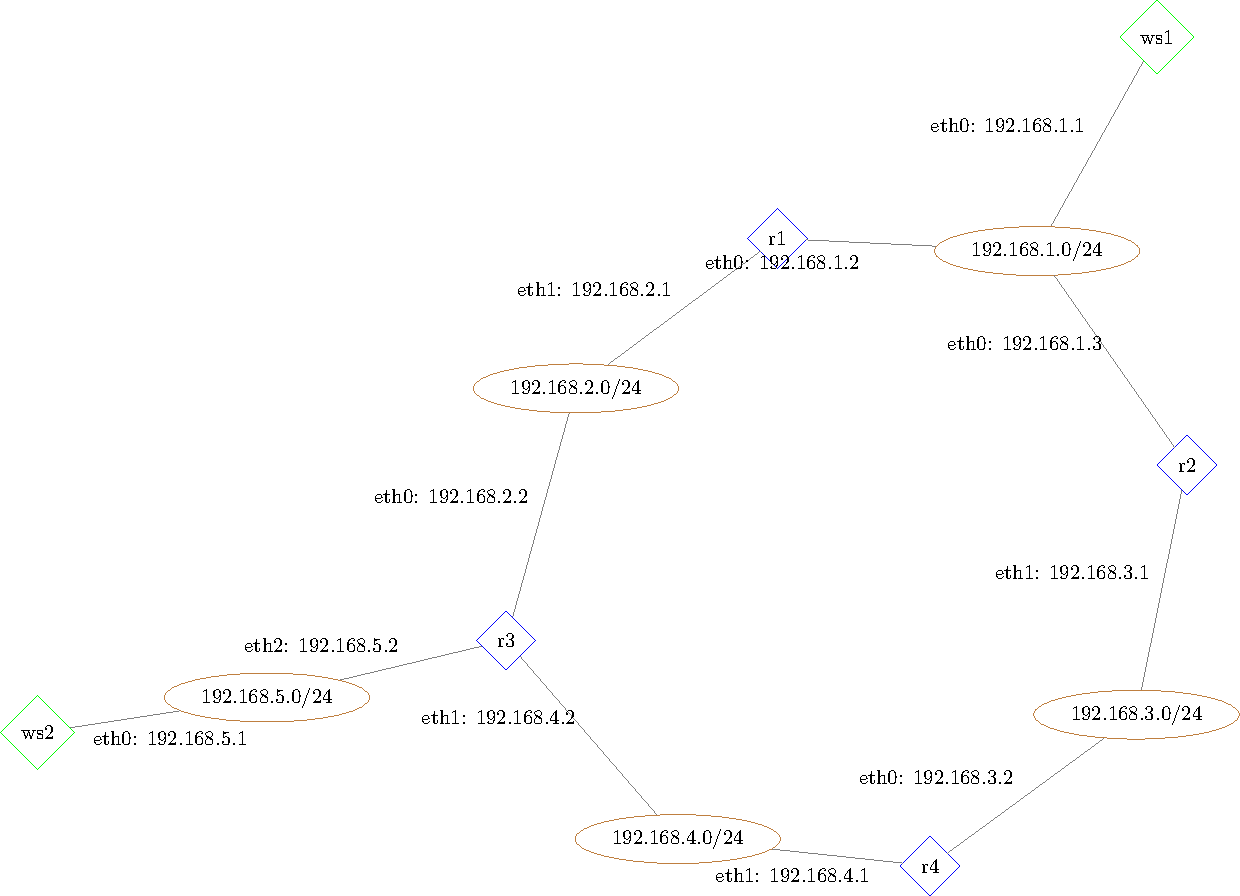
\includegraphics[width=\textwidth]{includes/network_gv.pdf}
\caption{Топология сети}
\label{fig:network}
\end{figure}


\section{Назначение IP-адресов}

Ниже приведён файл настройки протокола IP маршрутизатора (указать, какого).

\begin{Verbatim}
Сюда нужно поместить характерный /etc/network/interfaces маршрутизатора
\end{Verbatim}

Ниже приведён файл настройки протокола IP рабочей станции (указать, какой).

\begin{Verbatim}
Сюда нужно поместить характерный /etc/network/interfaces рабочей станции
\end{Verbatim}


\section{Таблица маршрутизации}

Вывести (командой ip r) таблицу маршрутизации для \textbf{r1}.

\begin{Verbatim}
Таблица маршрутизациии здесь
\end{Verbatim}

Вывести (командой ip r) таблицу маршрутизации для \textbf{r2}.

\begin{Verbatim}
Таблица маршрутизациии здесь
\end{Verbatim}

% ... Повторять для всех маршрутизаторов и рабочих станций, где есть что-то кроме gateway.

\section{Проверка настройки сети}

Вывод \textbf{traceroute} от узла такого-то до такого-то при нормальной работе сети.

\begin{Verbatim}
Сюда нужно поместить вывод traceroute.
\end{Verbatim}

Вывод \textbf{traceroute} от узла такого-то до такого-то при нормальной работе сети.

\begin{Verbatim}
Сюда нужно поместить вывод traceroute.
\end{Verbatim}

Вывод \textbf{traceroute} от узла такого-то до такого-то при нормальной работе сети.

\begin{Verbatim}
Сюда нужно поместить вывод traceroute.
\end{Verbatim}


\section{Маршрутизация}

% На пути здесь достаточно быть одному аршрутизатору!

Вначале стоит написать, какие MAC-адреса интерфейсов в опыте были у каких машин.
Затем вывести маршрутную таблицу маршрутизатора (вывод команды ip r!)

\begin{Verbatim}
маршрутная таблица маршрутизатора
\end{Verbatim}

Показаны опыты после стирания кеша ARP.
% Не забудьте это сделать!
Далее показана отправка пакета на маршрутизатор (косвенная маршрутизация). 

\begin{Verbatim}
Тут должен быть виден arp и затем посылка пакета маршрутизатору. 
С мак-адресами.
\end{Verbatim}

Затем маршрутизатор отправил его далее.

\begin{Verbatim}
Тут должен быть виден arp и затем посылка пакета маршрутизатором конечному получателю. 
С мак-адресами.
\end{Verbatim}

\section{Продолжительность жизни пакета}

Сначала написать как и на чём ломали. 

\begin{Verbatim}
Команды ломания
\end{Verbatim}

Потом какая-то таблица вышла.

\begin{Verbatim}
Испорченная таблица маршрутизации
\end{Verbatim}

Потом что слали.

\begin{Verbatim}
Команда посылки
\end{Verbatim}

И что в итоге получилось.

\begin{Verbatim}
Чуть сокращеннный лог, с мак адресами
\end{Verbatim}

И кто в итоге отравил сообщение о завершении жизни.

\section{Изучение IP-фрагментации}

Написать, на каких узлах и как изменяли MTU.


\begin{Verbatim}
Изменение MTU
\end{Verbatim}

\begin{Verbatim}
Изменение MTU
\end{Verbatim}

% Напоминаем, что PMTU следует отключить!

Какие команды давали для тестирования и где.

\begin{Verbatim}
Здесь вписать команду
\end{Verbatim}

Вывод \textbf{tcpdump} на маршрутизаторе перед сетью с уменьшенным MTU.

% Вывод в ширину можно и сократить, удалив несущественные моменты!

\begin{Verbatim}
Здесь вывод tcpdump, мак адреса не нужны.
\end{Verbatim}

Вывод \textbf{tcpdump} на маршрутизаторе после сети с уменьшенным MTU.

% Вывод в ширину можно и сократить, удалив несущественные моменты!

\begin{Verbatim}
Здесь вывод tcpdump, мак адреса не нужны.
\end{Verbatim}


Вывод \textbf{tcpdump} на узле получателя.

\begin{Verbatim}
Здесь вывод tcpdump, мак адреса не нужны.
\end{Verbatim}


\section{Отсутствие сети}

Аналогично опишите опыт, когда маршрутизатор отсылает сообщение об отстутствии с сети.
С командами и выводом, мак адреса не нужны.


\section{Отсутствие IP-адреса в сети}

Аналогично опишите опыт, когда маршрутизатор отсылает сообщение об отстутствии требуемого IP-адреса в сети.
С командами и выводом, мак адреса не нужны.

\end{document}
